\newpage
\thispagestyle{sectioned}
\chapter{Estado del Arte}

\section{Servidor: Wave}

\section{Aplicación Android: DemoCritics}

En esta sección exploraremos algunas de las principales aplicaciones informáticas que existen en la actulidad destinadas a la participación ciudadana en propuestas, lectura de programas electorales o divulgación de candidaturas.

\subsection{Programas Políticos}

En la actualidad no existe ningún tipo de aplicación móvil orientada a debatir los programas electorales de los partidos políticos en su conjunto. Concretamente no existe ningún tipo de plataforma que agrupe en un solo sitio los programas electorales de las diferentes candidaturas.
Lo más parecido que hemos podido encontrar han sido aplicaciones elaboradas por un partido político, orientadas a dar a conocer su candidatura. En ellas podemos ver normalmente, entre otros, a presentación de candidatura, vídeos propagandísticos y el programa electoral. 

Pasamos ahora a analizar algunas de las aplicaciones móviles encontradas, identificando en cada caso aspectos e ideas que nos han resultado positivos y negativos.

\subsubsection{UPyD Parla}
La aplicación presenta al candidato de UpyD Carlos Alt Bustelo para la alcaldía de Parla. Se trata de una alicación divulgativa donde podemos conocer todo lo esencial de la candidatura de UpyD para las elecciones del municipio de Parla en Mayo de 2015: los candidatos, el programa, vídeos, etc.

\begin{figure}[H]
        \centering
        \begin{subfigure}[b]{0.3\textwidth}
                \includegraphics[width=\textwidth]{Media/Captures/UPyDParlaIndex.jpg}
                \caption{Indice Programa}
                \label{fig:upydIndex}
        \end{subfigure}
        ~
        \begin{subfigure}[b]{0.3\textwidth}
                \includegraphics[width=\textwidth]{Media/Captures/UPyDParlaSection.jpg}
                \caption{Sección Programa}
                \label{fig:upydSection}
        \end{subfigure}
        ~
        \begin{subfigure}[b]{0.3\textwidth}
                \includegraphics[width=\textwidth]{Media/Captures/UPyDParlaCandidates.jpg}
                \caption{Candidatos}
                \label{fig:upydCandidates}
        \end{subfigure}
        \caption{Capturas de UPyD Parla}\label{fig:upydCaptures}
\end{figure}

 - \underline{Aspectos positivos}:

\begin{itemize}
	\item Interfaz limpia y de colores planos (predominando el rosa que identifica al partido) con menú lateral que permite navegar por la aplicación estés donde estés.
	\item Presentación de Programa Electoral estructurado con Indice inicial.
	\item El Programa se lee dentro de la app, no nos lleva a leer el programa en PDF de la web. 
	\item Presentación de una Sección del Programa Electoral de forma resumida, teniendo la opción de leer la sección entera al pulsar un botón.
\end{itemize}

 - \underline{Aspectos negativos}:

\begin{itemize}
	\item Posee una sección llamada ''Memes'' cuyo nombre no se entiende ya que se limita a mostrar carteles propagandísticos de la candidatura. 
\end{itemize}

\subsubsection{$\sharp$RecuperaCórdoba}
Esta app presenta la candidatura de Pedro García de Izquierda Unida a la provincia de Córdoba, informando de su propuesta de gobierno de forma resumida. En la aplicación podremos encontrar la lista de los candidatos propuestos a la comunidad cordobesa, el programa electoral de la formación, las propuestas del partido, noticias de última hora y vídeos.

\begin{figure}[H]
        \centering
        \begin{subfigure}[b]{0.3\textwidth}
                \includegraphics[width=\textwidth]{Media/Captures/IURecuperaCordoba.jpg}
                \caption{Indice Programa}
                \label{fig:iuIndex}
        \end{subfigure}
        ~
        \begin{subfigure}[b]{0.3\textwidth}
                \includegraphics[width=\textwidth]{Media/Captures/IURecuperaCordobaSection.jpg}
                \caption{Sección Programa}
                \label{fig:iuSection}
        \end{subfigure}
        ~
        \begin{subfigure}[b]{0.3\textwidth}
                \includegraphics[width=\textwidth]{Media/Captures/IURecuperaCordobaCandidates.jpg}
                \caption{Candidatos}
                \label{fig:iuCandidates}
        \end{subfigure}
        \caption{Capturas de $\sharp$IURecuperaCórdoba}
        \label{fig:iuRecuperaCordoba}
\end{figure}

 - \underline{Aspectos positivos}:

\begin{itemize}
	\item 
\end{itemize}

 - \underline{Aspectos negativos}:

\begin{itemize}
	\item 
\end{itemize}

\subsubsection{PSOE Andalucía}

Esta app presenta la candidatura del PSOE a la junta de Andalucía para las elecciones del 22 de Marzo, promocionando básicamente su programa electoral y a la candidata Susana Díaz. Permite también estar al día de noticias y eventos relacionados con dicha candidatura.

La navegación por el programa, aunque estructurada en un primer nivel, se realiza directamente visualizando páginas que parecen extraidas del programa en PDF.

\begin{figure}[H]
        \centering
        \begin{subfigure}[b]{0.3\textwidth}
                \includegraphics[width=\textwidth]{Media/Captures/psoeAndalucia.jpg}
                \caption{Pantalla Principal}
                \label{fig:psoePpal}
        \end{subfigure}
        ~
        \begin{subfigure}[b]{0.3\textwidth}
                \includegraphics[width=\textwidth]{Media/Captures/psoeAndaluciaIndex.jpg}
                \caption{Indice Programa}
                \label{fig:psoeIndex}
        \end{subfigure}
        ~
        \begin{subfigure}[b]{0.3\textwidth}
                \includegraphics[width=\textwidth]{Media/Captures/psoeAndaluciaSection.jpg}
                \caption{Sección Programa}
                \label{fig:psoeSection}
        \end{subfigure}
        \caption{Capturas de PSOE Andalucia}
        \label{fig:psoeAndalucia}
\end{figure}

 - \underline{Aspectos positivos}:

\begin{itemize}
	\item 
\end{itemize}

 - \underline{Aspectos negativos}:

\begin{itemize}
	\item 
\end{itemize}

\subsubsection{PP Canarias}

La delegación del Partido Popular en Canarias presenta su aplicación móvil para promocionar a sus candidatos para las elecciones autonómicas y municipales de Mayo de 2015. La aplicación nos avisará de los eventos electorales, podremos consultar los candidatos, novedades, galería de imágenes y por supuesto ver el programa electoral.

\begin{figure}[H]
        \centering
        \begin{subfigure}[b]{0.3\textwidth}
                \includegraphics[width=\textwidth]{Media/Captures/ppCanarias.jpg}
                \caption{Pantalla Principal}
                \label{fig:ppIndex}
        \end{subfigure}
        ~
        \begin{subfigure}[b]{0.3\textwidth}
                \includegraphics[width=\textwidth]{Media/Captures/ppCanariasProgram.jpg}
                \caption{Programas}
                \label{fig:ppPrograms}
        \end{subfigure}
        ~
        \begin{subfigure}[b]{0.3\textwidth}
                \includegraphics[width=\textwidth]{Media/Captures/ppCanariasCandidates.jpg}
                \caption{Candidatos}
                \label{fig:ppCandidates}
        \end{subfigure}
        \caption{Capturas de PP Canarias}
        \label{fig:ppCanarias}
\end{figure}

 - \underline{Aspectos positivos}:

\begin{itemize}
	\item 
\end{itemize}

 - \underline{Aspectos negativos}:

\begin{itemize}
	\item 
\end{itemize}

\subsection{Participación Ciudadana} \label{ssec:artProposals}

Centrándonos en la participación ciudadana ya sea mediante la generación de Propuestas, el desarrollo colaborativo de programas o la recogida de firmas, existen numerosos portales en internet y aplicaciones móviles destinadas a ello. Realizaremos un breve repaso a las aplicaciones más destacadas.

\subsubsection{Reddit}

Reddit \cite{ref:reddit} es una plataforma web donde los usuarios pueden crear temas, propuestas o compartir enlaces web a otros sitios. A primera vista puede parecer un foro, aunque la principal diferencia respecto a éste último radica en que otros usuarios pueden votar a favor o en contra de los enlaces, haciendo que el sistema los haga aparecer como más o menos destacados. De esta forma los temas de conversación, enlaces, o propuestas aparecerán en el orden que haya escogido la comunidad según la puntuación positiva o negativa que le hayan dado.
En principio el uso de reddit está destinado a todo tipo de temas, entre los que podemos encontrar algunos ejemplos fuertemente relacionados con la participación ciudadana. Es el caso de Plaza Podemos \cite{ref:plazaPodemos}: un espacio utilizado para que la ciudadanía pueda expresar sus propuestas, compartir noticias relacionadas con la actualidad política o debatir aquellos temas que más les preocupan. Así, aunque no seamos participantes de reddit, de un simple vistazo podemos saber qué es lo más debatido por la ciudadanía, las propuestas que quieren llevar a cabo en en el gobierno o cuáles son los temas que más les preocupan.

\begin{figure}[H]
\centering
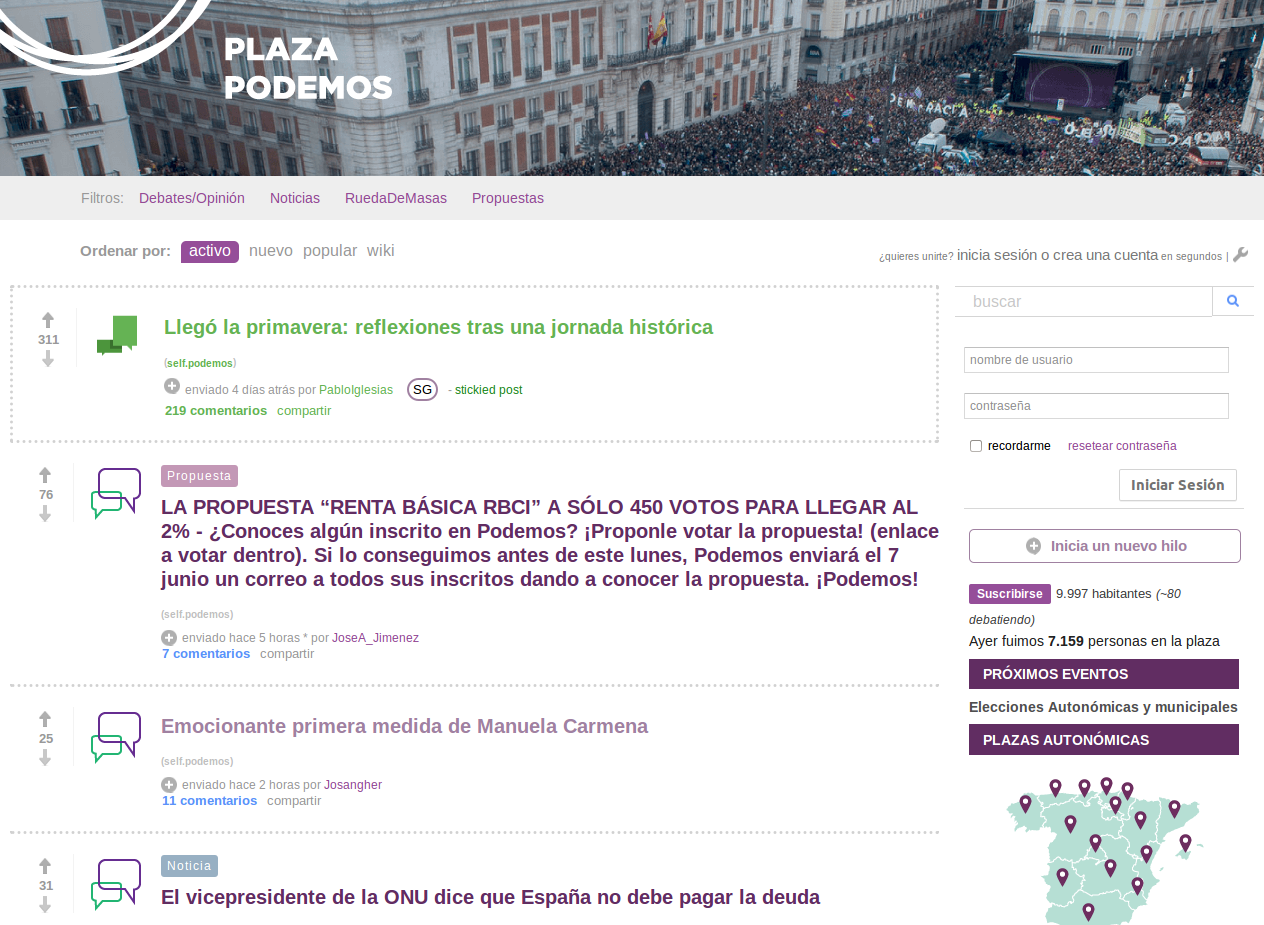
\includegraphics[keepaspectratio, scale=0.30]{Media/Captures/plazaPodemos.png}
\caption{Plaza Podemos utilizando la plataforma Reddit}
\label{fig:plazaPodemos}
\end{figure}

 - \underline{Aspectos positivos}:

\begin{itemize}
	\item 
\end{itemize}

 - \underline{Aspectos negativos}:

\begin{itemize}
	\item 
\end{itemize}

\subsubsection{Change.org}

Change.org \cite{ref:changeOrg} es un portal web que permite lanzar múltiples peticiones de cambio en Internet. Podríamos definirlo como la evolución de la recogida de firmas en la calle: cualquiera puede realizar una petición para solicitar el apoyo de otros. Las personas que decidan apoyar la petición, dejarán sus datos personales y constarán entre el número de personas que han firmado a favor de la petición. Una vez que han alcanzado un número objetivo de apoyos se procede a entregar las firmas digitales al organismo, persona o entidad a la que va destinada la petición.

Por ejemplo: en mayo de 2011, en relación con las movilizaciones del Movimiento 15-M y Democracia Real Ya, y ante el desalojo por los Mossos de Esquadra se llevó a cabo la petición “Exige la dimisión fulminante del Conseller de Interior Felip Puig por la violencia utilizada en Pza. Catalunya”.

Desde su creación en 2007, Change.org ha logrado muchas de sus peticiones demandadas entre los que se incluyen la atención de pacientes con enfermedades complejas, protección sobre animales y medio ambiente, derechos públicos, leyes, etc.

\begin{figure}[H]
\centering
\includegraphics[keepaspectratio, scale=0.30]{Media/Captures/changeOrg.png}
\caption{Change.org · La mayor plataforma de peticiones del mundo}
\label{fig:changeOrg}
\end{figure}

 - \underline{Aspectos positivos}:

\begin{itemize}
	\item 
\end{itemize}

 - \underline{Aspectos negativos}:

\begin{itemize}
	\item 
\end{itemize}

\subsubsection{Programas Colaborativos de Ahora Madrid y Zaragoza en Común}

Para las pasadas elecciones municipales del 24 de Mayo, la candidatura de unidad popular Ahora Madrid, desarrolló una plataforma en la web para elaborar su programa electoral de forma colaborativa. En esta plataforma, cualquier usuario tenía la oportunidad de explorar las propuestas por categoría o por distrito. De tal forma que podría debatirlas, puntuarlas o crear sus propias propuestas. Así las propuestas más valoradas por la comunidad, serían llevadas al programa final para las elecciones municipales del 24 de Mayo.

El resultado final fue determinar las cinco propuestas más votadas que fueron incluidas en el programa final como medidas urgentes para realizar en los 100 primeros días de gobierno. 

\begin{figure}[H]
\centering
\includegraphics[keepaspectratio, scale=0.25]{Media/Captures/programaAhoraMadrid.jpg}
\caption{Creación colaborativa del programa de Ahora Madrid.}
\label{fig:programaAhoraMadrid}
\end{figure}

También utilizaron una plataforma similar en la candidatura zaragozana de unidad popular Zaragoza en Común \cite{ref:ganemosZaragoza}.

\begin{figure}[H]
\centering
\includegraphics[keepaspectratio, scale=0.30]{Media/Captures/programaColaborativoGanemosZaragoza.png}
\caption{Creación colaborativa del programa de Zaragoza en Común.}
\label{fig:programaZaragozaEnComun}
\end{figure}

 - \underline{Aspectos positivos}:

\begin{itemize}
	\item 
\end{itemize}

 - \underline{Aspectos negativos}:

\begin{itemize}
	\item 
\end{itemize}

\subsubsection{Appgree}

Appgree\cite{ref:appgree} es una plataforma desarrollada con el objetivo de poner a grandes grupos de personas de acuerdo en poco tiempo. Está disponible tanto para web como para móviles y permite que sus usuarios lancen propuestas y debatan sobre cualquier tema pudiendo votar y alcanzar un consenso, obteniendo los resultados de dicha votación casi en tiempo real gracias a un algoritmo estadístico desarrollado por ellos llamado DemoRank\cite{ref:appgree_demoRank}.

En la aplicación podemos acceder a una lista de canales: que aglutinan encuestas, propuestas y preguntas (ya sea de respuesta abierta o de votación entre dos o mas opciones), pudiendo votar y ver los resultados actuales de votación y respuestas. Para fomentar la participación potencian mucho el uso tops de preguntas más candentes y recientes. Además se pueden compartir preguntas por redes sociales para aumentar su difusión.

\begin{figure}[H]
        \centering
        \begin{subfigure}[b]{0.3\textwidth}
                \includegraphics[width=\textwidth]{Media/Captures/appgreeChannel.jpg}
                \caption{Canal}
                \label{fig:appgreeChannel}
        \end{subfigure}
        ~
        \begin{subfigure}[b]{0.3\textwidth}
                \includegraphics[width=\textwidth]{Media/Captures/appgreeQuestion.jpg}
                \caption{Pregunta Múltiple}
                \label{fig:appgreeQuestion}
        \end{subfigure}
        ~
        \begin{subfigure}[b]{0.3\textwidth}
                \includegraphics[width=\textwidth]{Media/Captures/appgreeOpenQuestion.jpg}
                \caption{Pregunta Abierta}
                \label{fig:appgreeOpenQuestion}
        \end{subfigure}
        \caption{Capturas de Appgree}\label{fig:appgreeCaptures}
\end{figure}

 - \underline{Aspectos positivos}:

\begin{itemize}
	\item 
\end{itemize}

 - \underline{Aspectos negativos}:

\begin{itemize}
	\item 
\end{itemize}
